In diesem Abschnitt werden die erzielten Ergebnisse des Projekts beschrieben und kritisch bewertet. 
Der Fokus liegt auf der funktionalen Umsetzung, der Leistungsbewertung des Systems und einer Analyse 
der Stärken und Schwächen.

\subsection{Funktionale Ergebnisse}

Das Projektziel, einen voll funktionsfähigen Prototypen für einen smarten Cocktailautomaten zu 
entwickeln, wurde erfolgreich erreicht. Die wesentlichen funktionalen Anforderungen konnten 
umgesetzt werden:

\begin{itemize}
  \item \textbf{Automatisierte Cocktailzubereitung:} Die Hardware steuert präzise die Pumpen und 
  Motoren, um Zutaten gemäß den Rezeptvorgaben abzugeben.
  \item \textbf{Mobile App:} Benutzer können über eine intuitive App Rezepte erstellen, verwalten 
  und Bestellungen auslösen.
  \item \textbf{Backend-Integration:} Das Backend verarbeitet Bestellungen zuverlässig, 
  \\synchronisiert Benutzerdaten und leitet Steuerbefehle an die Hardware weiter.
\end{itemize}

Die abschließenden Integrationstests zeigten, dass das Gesamtsystem von der Rezeptbestellung in der 
App bis zur Zubereitung durch die Hardware stabil funktioniert.

\subsection{Leistungsbewertung der Pumpen}

Der Test der Pumpen ergab, dass die Dosiergenauigkeit der einzelnen Pumpen mitunter Stark abweicht. 
Die Leistung der Pumpen ist in Abbildung \ref{fig:pump_performance} dargestellt. Grund für das 
Abweichen der Pumpen 1 und 5 ist vermutlich ein Defekt durch eine anfänglich unsachgemäße 
Inbetriebnahme unsererseits. Die Pumpen 2, 3, 4 und 6 zeigen eine gute Leistung und eine geringe 
Abweichung. Die Pumpen 2, 3 und 4 sind dabei besonders genau und weisen eine geringe Abweichung auf.

Die Probleme der Pumpen lassen sich jedoch mittels einer Kalibrierung des Pumpfaktors beheben. 
Alternativ kann auch eine Zukünftige Verwendung der Waage das Problem beheben, da die Waage die
tatsächlich ausgegebene Menge misst und die Pumpen entsprechend rechtzeitig gestoppt werden können.

\begin{figure}[H] 
    \centering 
    \begin{tikzpicture} 
        \begin{axis}[ 
            boxplot/draw direction=y, 
            ylabel={ Menge in Milliliter }, % Beschriftung der y-Achse 
            xlabel={ Pumpen }, % Beschriftung der x-Achse
            xtick={ 1, 2, 3, 4, 5, 6 }, % Positionen der xticks 
            xticklabels={ 1, 2, 3, 4, 5, 6 }, % Labels der xticks
            ymin=210, 
            ymax=430, % Begrenzung der y-Achse 
            boxplot/every box/.style={solid}
            ] 
            \addplot [ 
                thick, dashed, blue, 
                domain=0:7, 
            ] {400}; 
            \addplot+ [ boxplot, fill=red4, draw=red7, solid ] 
            table[row sep=\\, y index=0] 
            { 
                370 \\ 375 \\ 357 \\ 364 \\ 358 \\ 362 \\ 382 \\ 383 \\ 370 \\ 366 \\ 370 \\ 368 \\ 
                383 \\ 373 \\ 360 \\ 355 \\ 373 \\ 381 \\ 356 \\ 349 \\ 362 \\ 370 \\ 369 \\ 361 \\ 
            }; 
            \addplot+ [ boxplot, fill=red4, draw=red7, solid ] 
            table[row sep=\\, y index=0] 
            { 
                399 \\ 388 \\ 395 \\ 395 \\ 399 \\ 409 \\ 402 \\ 400 \\ 386 \\ 401 \\ 400 \\ 400 \\ 
                404 \\ 387 \\ 405 \\ 400 \\ 400 \\ 390 \\ 388 \\ 400 \\ 400 \\ 399 \\ 405 \\ 399 \\ 
            }; 
            \addplot+ [ boxplot, fill=red4, draw=red7, solid ] 
            table[row sep=\\, y index=0] 
            { 
                397 \\ 402 \\ 395 \\ 398 \\ 400 \\ 400 \\ 395 \\ 400 \\ 402 \\ 400 \\ 399 \\ 408 \\ 
                395 \\ 388 \\ 403 \\ 400 \\ 402 \\ 400 \\ 408 \\ 388 \\ 396 \\ 408 \\ 397 \\ 390 \\ 
            }; 
            \addplot+ [ boxplot, fill=red4, draw=red7, solid ]
            table[row sep=\\, y index=0] 
            { 
                411 \\ 400 \\ 398 \\ 399 \\ 400 \\ 408 \\ 408 \\ 415 \\ 400 \\ 386 \\ 393 \\ 390 \\ 
                400 \\ 404 \\ 400 \\ 406 \\ 409 \\ 400 \\ 403 \\ 396 \\ 406 \\ 407 \\ 405 \\ 396 \\ 
            };
            \addplot+ [ boxplot, fill=red4, draw=red7, solid ] 
            table[row sep=\\, y index=0] 
            { 
                267 \\ 259 \\ 305 \\ 242 \\ 306 \\ 315 \\ 313 \\ 287 \\ 266 \\ 300 \\ 298 \\ 260 \\
                285 \\ 251 \\ 283 \\ 243 \\ 266 \\ 263 \\ 255 \\ 278 \\ 241 \\ 255 \\ 315 \\ 280 \\ 
            }; 
            \addplot+ [ boxplot, fill=red4, draw=red7, solid ] 
            table[row sep=\\, y index=0] 
            { 
                382 \\ 385 \\ 387 \\ 382 \\ 390 \\ 386 \\ 390 \\ 377 \\ 393 \\ 388 \\ 383 \\ 398 \\ 
            }; 
        \end{axis}
    \end{tikzpicture} 
    \caption{Pumpenleistung für 400ml} 
    \label{fig:pump_performance} 
\end{figure}

\subsection{Lasttestergebnisse und Analyse}

Zur Bewertung der Performance und Skalierbarkeit des Systems wurden umfassende Lasttests mit dem 
Tool \texttt{k6} durchgeführt. Diese Tests simulierten eine Vielzahl gleichzeitiger 
Benutzeranfragen, um Engpässe und Optimierungspotenziale zu identifizieren. Die wichtigsten 
Ergebnisse sind im Folgenden zusammengefasst.

\subsubsection*{Gesamtergebnisse}

\subsubsection*{Wichtige Metriken}
\begin{itemize}
    \item \textbf{Gesamtanfragen:} 16.506
    \item \textbf{Fehlerrate:} 0,08\% (14 fehlgeschlagene Anfragen)
    \item \textbf{Durchschnittliche Antwortzeit:} 274,48 ms
    \item \textbf{Minimale Antwortzeit:} 13,87 ms
    \item \textbf{Median der Antwortzeit:} 19,75 ms
    \item \textbf{Maximale Antwortzeit:} 282.415,99 ms
    \item \textbf{90. Perzentil der Antwortzeit:} 78,66 ms
    \item \textbf{95. Perzentil der Antwortzeit:} 121,84 ms
\end{itemize}

% ERFOLGSRATE --------------------------------------------------------------------------------------
\subsubsection*{Erfolgsrate}

\begin{table}[H]
    \centering
    % \resizebox{\textwidth}{!}{%
        \begin{tabular}{|l|r|r|r|}
            \hline
            \textbf{Test} & \textbf{Erfolgreich} & \textbf{Fehlgeschlagen} & \textbf{Erfolgsrate} \\
            \hline
            Nutzerregistrierung   &  263 &   0 &  100\% \\
            Nutzer einloggen      &  263 &   0 &  100\% \\
            Hardwareregistrierung &  262 &   1 &   99\% \\
            Drink erstellen       & 2615 &   5 &   99\% \\
            Slot setzen           & 1304 &   6 &   99\% \\
            Rezept erstellen      & 2619 &   1 &   99\% \\
            Zutat hinzufügen      & 2620 &   0 &  100\% \\
            Favorit erstellen     &  785 &   1 &   99\% \\
            Slots abfragen        &  262 &   0 &  100\% \\
            Favoriten abfragen    &  263 &   0 &  100\% \\
            \hline
        \end{tabular}
    % }
    \caption{Tests je Endpunkt und Erfolgsrate}
    \label{tab:test_success_rate}    
\end{table}

Die Erfolgsrate der einzelnen API-Endpunkte ist insgesamt hoch. Die Nutzerregistrierung und das 
Einloggen waren zu 100\% erfolgreich, während die Hardwareregistrierung eine Erfolgsrate von 99\% 
aufweisen. Die Fehlerrate bei der Erstellung von Getränken und Rezepten, dem setzen von Slots und 
dem hinzufügen von Bestandteilen zu einem Rezept liegt bei 1\%. Diese Fehler lassen sich aber 
allesamt durch das Fehlschlagen der Hardwareregistrierung erklären, da diese für einen Eintrag in 
die Datenbank benötigt wird. Die Erfolgsrate der Favoritenfunktion liegt aus dem selben Grund 
lediglich bei 99\%. Alles in allem sind die Ergebnisse zufriedenstellend. 
Das scheitern der Hardware registrieren Anfrage ist auf eine Auslastung der Container Instanz 
zurückzuführen, und könnte mit mehr Leistung, mit weiteren Container Instanzen oder einer 
Optimierung der Anfrage behoben werden.

% ANTOWRTZEITEN ------------------------------------------------------------------------------------
\subsubsection*{Antwortzeiten pro Endpunkt}

Die Antwortzeiten für spezifische API-Endpunkte zeigen deutliche Unterschiede, die auf 
unterschiedliche Verarbeitungskomplexität hinweisen. Die wichtigsten Werte sind in Tabelle 
\ref{tab:response_times} dargestellt.

\begin{table}[H] 
    \centering
    % \resizebox{\textwidth}{!}{%
        \begin{tabular}{|l|r|r|r|r|}
            \hline
            \textbf{Endpunkt} &
            \textbf{Durchschnitt} & 
            \textbf{Median} & 
            \textbf{90. Perzentil} & 
            \textbf{Max} \\
            \hline
            Nutzer registrieren     &  145,60 & 102,70 & 219,23 &   1224,98 \\
            Nutzer einlogen         &  155,90 & 102,51 & 283,79 &   1530,31 \\
            Hardware registrieren   & 1241,48 &  70,54 & 218,08 & 282415,99 \\
            Drink erstellen         &  588,13 &  19,39 &  52,83 & 282275,98 \\
            Rezept erstellen        &  136,98 &  19,10 &  42,42 & 282282,60 \\
            Zutat hinzufügen        &   29,39 &  18,85 &  46,66 &    422,70 \\
            Slot setzen             & 1341,94 &  23,35 &  79,69 & 282292,87 \\
            Rezept favorisieren     &  268,85 &  24,01 &  64,44 & 183405,20 \\
            Alle Favoriten abfragen &   29,58 &  20,01 &  51,67 &    227,09 \\
            Slotbelegung abfragen   &   64,92 &  48,96 & 112,32 &    355,33 \\
            \hline
        \end{tabular}
    % }
    \caption{Antwortzeiten je Endpunkt in Millisekunden}
    \label{tab:response_times}
\end{table}

Bei einer genaueren Betrachtung der Antwortzeiten pro Endpunkt fällt auf, dass die Endpunkte mit 
den höchsten Maximalwerten (Hardware registrieren, Drink erstellen, Rezept erstellen, Slot setzen, 
Favorit setzen) wieder die selben Punkte sind welche bereits zuvor als fehleranfällig identifiziert
wurden. Die Antwortzeiten sind in diesen Fällen sehr hoch, was auf eine Überlastung der Container 
Instanz zurückzuführen ist. Die Antwortzeiten der anderen Endpunkte sind im Vergleich dazu sehr
gering. Die Antwortzeiten der Endpunkte Zutat hinzufügen, Alle Favoriten abfragen und Slotbelegung
abfragen sind besonders niedrig, was auf eine geringe Verarbeitungskomplexität hinweist.

\hyphenation{Live-Umgebung}
\hyphenation{Web-socket-Ver-bind-ung}
Die Tests haben gezeigt, dass das System in einer Live-Umgebung grundsätzlich stabil arbeitet. 
Allerdings wurden Skalierungsprobleme bei Websocket-Verbindungen identifiziert, die durch eine 
zentrale Verwaltung oder eine konsistente Lastverteilung gelöst werden könnten. Die meisten API-
Endpunkte zeigten zufriedenstellende Antwortzeiten und Erfolgsquoten. Die Schwachstellen bieten 
jedoch Anknüpfungspunkte für zukünftige Optimierungen.

% USABILITY ----------------------------------------------------------------------------------------
\subsection{User-Test Ergebnisse}

Zur Evaluation der Benutzerfreundlichkeit, des Funktionsumfangs und der Stabilität der mobilen App 
wurden neun Personen eingeladen, die App zu testen. Sie bewerteten die App in den drei Kategorien 
auf einer Skala von 1 (schlecht) bis 5 (sehr gut). Die Ergebnisse sind in Tabelle 
\ref{tab:user_tests} und in der Visualisierung in Abbildung \ref{fig:user_tests2} dargestellt.

\begin{table}[h!]
    \centering
    \begin{tabular}{|l|c|}
        \hline
        \textbf{Kategorie} & \textbf{Durchschnittliche Bewertung} \\
        \hline
        Benutzerfreundlichkeit & 4,44 \\
        Funktionsumfang & 4,22 \\
        Stabilität und Leistung & 4,88 \\
        \hline
    \end{tabular}
    \caption{Ergebnisse der Benutzerbewertungen}
    \label{tab:user_tests}
\end{table}

\begin{figure}[h!]
    \centering
    \begin{minipage}{0.80\textwidth}
        \centering
        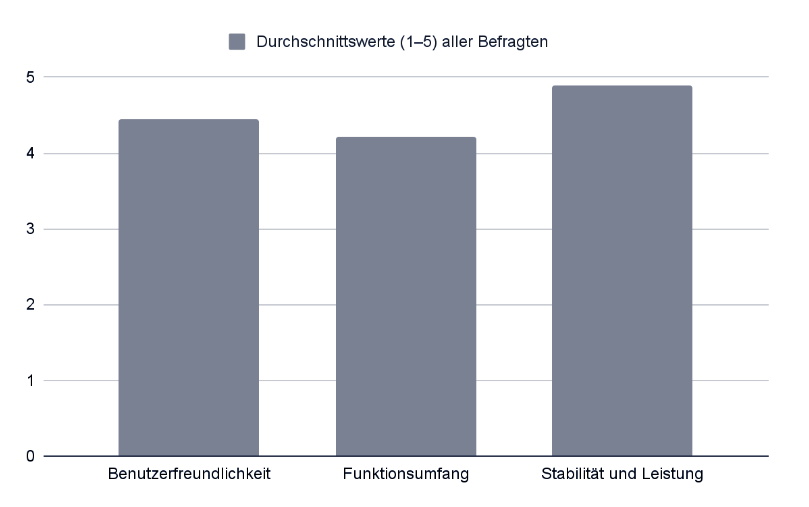
\includegraphics[width=\textwidth]{graphics/images/usertests_app.png}
        \caption{Usertest}
        \label{fig:user_tests2} % Direkt nach der caption setzen
    \end{minipage}
\end{figure}


\subsection{Stärken und Schwächen}

\subsubsection{Stärken}

Das Projekt weist folgende Stärken auf:
\begin{itemize}
  \item \textbf{Benutzerfreundlichkeit:} Die App bietet eine intuitive Benutzeroberfläche und 
  ermöglicht eine einfache Verwaltung von Rezepten und Geräten.
  \item \textbf{Technische Umsetzung:} Die Kombination aus App, Backend und Hardware zeigt das 
  Potenzial von IoT-Technologien in Smart-Home-Umgebungen.
  \item \textbf{Modularität:} Die Architektur des Systems ermöglicht zukünftige Erweiterungen, z. B. 
  die Integration zusätzlicher Geräte oder neue Funktionen.
\end{itemize}

\subsubsection*{Schwächen}

Einige Schwächen des aktuellen Prototyps wurden identifiziert:
\begin{itemize}
  \item \textbf{Skalierbarkeit:} Die Verwaltung von Websocket-Verbindungen in einer 
  containerisierten Umgebung führte bei hoher Last zu Problemen.
  \item \textbf{Fehlende Tests:} Es wurden keine umfassenden automatisierten Tests für die einzelnen 
  Systemkomponenten implementiert.
  \item \textbf{Hardware:} Obwohl die Hardware zuverlässig arbeitet, könnten Optimierungen in der 
  Dosiergenauigkeit und Stabilität vorgenommen werden.
\end{itemize}

\subsection{Zusammenfassung der Ergebnisse}

Das Projekt hat gezeigt, dass IoT-Technologien erfolgreich zur Automatisierung von Alltagsaufgaben 
eingesetzt werden können. Die entwickelten Systeme arbeiten zuverlässig und erfüllen die definierten 
funktionalen Anforderungen. Gleichzeitig wurden Schwächen aufgedeckt, die als Grundlage für 
zukünftige Optimierungen dienen können.

\subsection{Empfehlungen}
\hyphenation{Web-socket-Ser-ver}
Auf Basis der Testergebnisse und identifizierten Schwächen werden folgende Maßnahmen für zukünftige 
Verbesserungen empfohlen:
\begin{itemize}
  \item \textbf{Optimierung der Skalierung:} Einführung eines zentralen Websocket-Servers oder 
  konsistenter Lastverteilung, um Kommunikationsprobleme bei hoher Last zu beheben.
  \item \textbf{Automatisierte Tests:} Entwicklung und Implementierung umfassender \\
  Unit- und Integrationstests.
  \item \textbf{Hardware-Optimierungen:} Verbesserung der Dosiergenauigkeit und Integration 
  zusätzlicher Sensorik zur Überwachung.
\end{itemize}

% BOXPLOT PUMPEN -----------------------------------------------------------------------------------
\newpage
\begin{figure}[h!]
    \centering
    \begin{tikzpicture}
        \begin{axis}[
            boxplot/draw direction=y,
            ylabel={ Menge in Milliliter }, % Beschriftung der y-Achse
            xlabel={ Pumpen }, % Beschriftung der x-Achse
            xtick={ 1, 2, 3, 4, 5, 6 }, % Positionen der xticks
            xticklabels={ 1, 2, 3, 4, 5, 6 }, % Labels der xticks
            ymin=210, 
            ymax=430, % Begrenzung der y-Achse
            boxplot/every box/.style={solid}
        ]
        \addplot [
            thick, dashed, blue,
            domain=0:7, % Definiert den Bereich der x-Achse
        ] {400};
        \addplot+ [
            boxplot,
            fill=red4,
            draw=red7,
            solid
        ] table[row sep=\\, y index=0] {
            370 \\ 375 \\ 357 \\ 364 \\ 358 \\ 362 \\ 382 \\ 383 \\ 370 \\ 366 \\ 370 \\ 368 \\ 
            383 \\ 373 \\ 360 \\ 355 \\ 373 \\ 381 \\ 356 \\ 349 \\ 362 \\ 370 \\ 369 \\ 361 \\
        };
        \addplot+ [
            boxplot,
            fill=red4,
            draw=red7,
            solid
        ] table[row sep=\\, y index=0] {
            399 \\ 388 \\ 395 \\ 395 \\ 399 \\ 409 \\ 402 \\ 400 \\ 386 \\ 401 \\ 400 \\ 400 \\ 
            404 \\ 387 \\ 405 \\ 400 \\ 400 \\ 390 \\ 388 \\ 400 \\ 400 \\ 399 \\ 405 \\ 399 \\
        };
        \addplot+ [
            boxplot,
            fill=red4,
            draw=red7,
            solid
        ] table[row sep=\\, y index=0] {
            397 \\ 402 \\ 395 \\ 398 \\ 400 \\ 400 \\ 395 \\ 400 \\ 402 \\ 400 \\ 399 \\ 408 \\ 
            395 \\ 388 \\ 403 \\ 400 \\ 402 \\ 400 \\ 408 \\ 388 \\ 396 \\ 408 \\ 397 \\ 390 \\
        };
        \addplot+ [
            boxplot,
            fill=red4,
            draw=red7,
            solid
        ] table[row sep=\\, y index=0] {
            411 \\ 400 \\ 398 \\ 399 \\ 400 \\ 408 \\ 408 \\ 415 \\ 400 \\ 386 \\ 393 \\ 390 \\ 
            400 \\ 404 \\ 400 \\ 406 \\ 409 \\ 400 \\ 403 \\ 396 \\ 406 \\ 407 \\ 405 \\ 396 \\
        };
        \addplot+ [
            boxplot,
            fill=red4,
            draw=red7,
            solid
        ] table[row sep=\\, y index=0] {
            267 \\ 259 \\ 305 \\ 242 \\ 306 \\ 315 \\ 313 \\ 287 \\ 266 \\ 300 \\ 298 \\ 260 \\ 
            285 \\ 251 \\ 283 \\ 243 \\ 266 \\ 263 \\ 255 \\ 278 \\ 241 \\ 255 \\ 315 \\ 280 \\
        };
        \addplot+ [
            boxplot,
            fill=red4,
            draw=red7,
            solid
        ] table[row sep=\\, y index=0] {
            382 \\ 385 \\ 387 \\ 382 \\ 390 \\ 386 \\ 390 \\ 377 \\ 393 \\ 388 \\ 383 \\ 398 \\
        };
        \end{axis}

    \end{tikzpicture}
    \caption{Pumpenleistung für 400ml}
    \label{fig:pump_performance}
\end{figure}
\newpage
% --------------------------------------------------------------------------------------------------
% --------------------------------------------------------------------------------------------------
% --------------------------------------------------------------------------------------------------
% --------------------------------------------------------------------------------------------------
% --------------------------------------------------------------------------------------------------

\section*{Schlussfolgerungen}
Die Ergebnisse zeigen, dass:
\begin{itemize}
    \item Die Benutzerregistrierung und Rezeptverwaltung besonders fehleranfällig sind (nur 9\% 
        Erfolgsquote).
    \item Die API insgesamt eine hohe Fehlerrate von 45,11\% aufweist, was auf Skalierungs- oder 
        Ressourcenprobleme hindeuten könnte.
    \item Die durchschnittliche Antwortzeit (66,26 ms) akzeptabel ist, aber in Spitzenzeiten (max. 
        644 ms) stark ansteigt.
\end{itemize}

\section*{Empfehlungen}
\begin{itemize}
    \item Optimieren Sie die Ressourcen- und Skalierungseinstellungen von Google Cloud Run.
    \item Reduzieren Sie die Last in der Benutzerregistrierung durch bessere Datenbankabfragen 
        oder asynchrone Prozesse.
    \item Testen Sie kleinere Benutzergruppen, um die Schwellenwerte für Stabilitätsprobleme zu 
        identifizieren.
\end{itemize}
